%%%%%%%% ICML 2018 EXAMPLE LATEX SUBMISSION FILE %%%%%%%%%%%%%%%%%

\documentclass{article}

% Recommended, but optional, packages for figures and better typesetting:
\usepackage{microtype}
\usepackage{graphicx}
\usepackage{subfigure}
\usepackage{booktabs} % for professional tables

% my packages
\usepackage{amsmath}
\usepackage{amssymb}

% hyperref makes hyperlinks in the resulting PDF.
% If your build breaks (sometimes temporarily if a hyperlink spans a page)
% please comment out the following usepackage line and replace
% \usepackage{icml2018} with \usepackage[nohyperref]{icml2018} above.
\usepackage{hyperref}

% Attempt to make hyperref and algorithmic work together better:
\newcommand{\theHalgorithm}{\arabic{algorithm}}

% Use the following line for the initial blind version submitted for review:
\usepackage{icml2018}

% If accepted, instead use the following line for the camera-ready submission:
%\usepackage[accepted]{icml2018}

% The \icmltitle you define below is probably too long as a header.
% Therefore, a short form for the running title is supplied here:
\icmltitlerunning{Fully Autonomous First Order Mathematical Optimizer}

\begin{document}

\twocolumn[
\icmltitle{Fully Autonomous First Order Mathematical Optimizer}

% It is OKAY to include author information, even for blind
% submissions: the style file will automatically remove it for you
% unless you've provided the [accepted] option to the icml2018
% package.

% List of affiliations: The first argument should be a (short)
% identifier you will use later to specify author affiliations
% Academic affiliations should list Department, University, City, Region, Country
% Industry affiliations should list Company, City, Region, Country

% You can specify symbols, otherwise they are numbered in order.
% Ideally, you should not use this facility. Affiliations will be numbered
% in order of appearance and this is the preferred way.
%\icmlsetsymbol{equal}{*}

\begin{icmlauthorlist}
\icmlauthor{Animesh Karnewar}{ir}
\end{icmlauthorlist}

\icmlaffiliation{ir}{Independent Researcher}

\icmlcorrespondingauthor{Animesh Karnewar}{animeshsk3@gmail.com}

% You may provide any keywords that you
% find helpful for describing your paper; these are used to populate
% the "keywords" metadata in the PDF but will not be shown in the document
\icmlkeywords{Mathematical Optimization, First order optimization}

\vskip 0.3in
]

% this must go after the closing bracket ] following \twocolumn[ ...

% This command actually creates the footnote in the first column
% listing the affiliations and the copyright notice.
% The command takes one argument, which is text to display at the start of the footnote.
% The \icmlEqualContribution command is standard text for equal contribution.
% Remove it (just {}) if you do not need this facility.

%\printAffiliationsAndNotice{}  % leave blank if no need to mention equal contribution
\printAffiliationsAndNotice{} % otherwise use the standard text.

\begin{abstract}
This research paper describes a technique for performing mathematical optimization, which is free from any hyperparameters. The optimization requires only first order derivatives of the objective function with respect to the learning parameters. The step size, more commonly known as the learning rate, which is manually set for training is replaced by a heuristic which calculates an optimal step size relative to the instantaneous value of the objective function. Finally the results obtained on the MNIST dataset by using this technique are presented and discussed in brief while comparing to other optimization algorithms. The algorithm proves its stability on the MNIST classification and achieves performance comparable to Adam optimizer which is the current standard.
\end{abstract}

\section{Introduction}
\textbf{Mathematical Optimization} lies at the heart of Machine Learning. In order to statistically fit the function over the given data, the learnable parameters of the model are modified according to a certain objective function. This is true for both supervised and unsupervised learning. In case of the latter, the distinction is based only in the definition of the objective function, which in this case doesn’t involve any label information. The optimization is performed on a mathematical function \textit{f(x)} known as the \textbf{objective function} or \textbf{criterion} by obtaining the value of \textit{x} such that the value of \textit{f(x)} is optimal (either maximum or minimum). In general context, optimization refers to minimization of the criterion. The maximization of the same can be achieved by minimizing the negative criterion\textit{ -f(x)} \cite{goodfellow-et-al:deep-learning}. When the minimization is considered, the objective function is also referred to as \textbf{loss function} or \textbf{error function} or \textbf{cost function}.

\subsection{Related Works}
The \textbf{gradient descent} algorithm \cite{cauchy:gradient-descent} has been the most popular algorithm for performing mathematical optimization. It is an iterative algorithm which deduces the direction to move towards at any given particular instant by using the sign of the local gradient of \textit{f(x)} wrt \textit{x}. The update equation of gradient descent is given by:

\begin{center}
	$x_{t + 1} = x_{t} - \alpha $ $\cfrac{df(x_t)}{dx}$
\end{center}

where the $\alpha$ is known as the \textbf{learning rate} which specifies the step-size for any particular iteration of the algorithm. The most common method for choosing the value of $\alpha$ that has been applied is trial and run; and thereby the algorithm requires human attention.


Apart from its heavy reliance on a perfectly chosen learning rate, it was pointed out that the algorithm is susceptible to \textbf{ravines}, i.e. variable gradient rates along different dimensions \cite{sutton:gradient-descent-problems}. Over the years, various attempts have been made in order to patch up these flaws of the gradient descent algorithm. The use of \textbf{Momentum} in the update equation of gradient descent was an attempt at tackling the latter problem \cite{qian:momentum}. The update equations for the momentum are given by

\begin{center}
	$v_t = \gamma v_{t - 1} + (1 - \gamma) \cfrac{df(x_t)}{dx} $\\
	$x_{t + 1} = x_{t} - \alpha v_t$
\end{center}

where the $\gamma$ is known as the momentum weightage or the running average factor. In some literature, the $\gamma$ is also denoted by the symbol $\beta$, the meaning of both the symbols is however the same. The momentum modification takes into consideration the values of gradients of the previous iterations and accumulates them in the $v$ term. Unfortunately, in order to evade the problem of ravines, the momentum makes a trade off with the addition of another hyperparameter $\gamma$.


The Nesterov Accelrated Gradient or \textbf{NAG} \cite{nesterov:momentum} builds upon the concept of momentum and adds a future lookup via the accumulated gradients in order to make a better estimate of the optimal direction to move towards. The \textbf{RMSprop} optimization scales the current gradient by the inverse square root of accumulated second moments of the previous gradients. The current standard and the most widely employed algorithm \textbf{Adam} \cite{kingma-ba:adam} combines the concept of Momentum and RMSprop coupled with learning rate decay. The \textbf{Nadam} variant of the same, which uses the Nesterov Momentum, is also sometimes used for optimization. The systematic update equations of Adam are given by:

\begin{center}
	$g_t = \cfrac{d f(x_t)}{dx}$ \\
	$m_t = \beta_1 m_{t-1} + (1 - \beta_1) g_t$ \\
	$v_t = \beta_2 v_{t-1} + (1 - \beta_2) g_t^2$ \\
	$\hat{m_t} = \cfrac{m_t}{(1 - \beta_1^t)}$ \\
	$\hat{v_t} = \cfrac{v_t}{(1 - \beta_2^t)}$ \\
	$\hat{\alpha} = \alpha \cfrac{\sqrt{1 - \beta_2^t}}{1 - \beta_1^t}$ \\
	$x_{t + 1} = x_{t} - \hat{\alpha} \cfrac{\hat{m_t}}{(\sqrt{\hat{v_t}} + \epsilon)}$\\
\end{center}

There are in all four hyperparameters in the Adam update algorithm viz. $\alpha$, $\beta_1$, $\beta_2$ and $\epsilon$ of which, the $\epsilon$ is used for the numerical stability of the algorithm and is rarely tweaked. The default value used for $\epsilon$ is \textit{1e-8}.


There are various other algorithms that have been devised for the problem of Mathematical Optimization and have been utilised with varying rates of success; whereby, they all have their own advantages as well as shortcomings \cite{rudder:overview}. Some approaches based on statistical schedules such as \cite{darken:schedule} and using annealing \cite{robbins:annealing} have been published. Novel approaches such as the \cite{koolen:learning-learning-rate} and \cite{schaul:pesky} for the \textbf{stochastic gradient setting}, where update is made per data example, prominently stand out, but unfortunately it is felt that they add up redundant complexity to the task of Mathematical Optimization. Works that involve the use of \textit{\textbf{Higher Order Derivatives}} or \textit{\textbf{Hessians}} in the update equations that follow the lines of \textbf{Newton's Method} are not relevant to the present research and hence not compared.

\subsection{Comparative analysis}
In almost all these gradient descent variants, it occurs that as much of efforts that have been put towards making the algorithm stabler and more performant, have entailed increment of hyperparameters to the update equations, resulting in lesser autonomy. The statistical approaches that guide the selection of these hyperparameters fit the relevant domains perfectly but require the same efforts to be reproduced for disparate domains. This brings to highlight the two key factors of the optimization algorithm to be presented here: \textbf{simplicity} due to the use of only first order derivatives and simplistic geometric approximations without any momentum accumulation; and \textbf{autonomy} because of not requiring any hyperparameters; while making only one assumption about the loss function being positive real valued \footnote{The loss function for all the Machine Learning and Deep Learning tasks are almost always defined as positive real valued functions}.

\section{Mathematical explanation of the Algorithm}
This section provides a step by step description of the proposed algorithm for performing Mathematical Optimization.
Following sub-sections would present the update equation of the algorithm and also explain the mathematics supporting it. Followed by, the analysis of the parameter update portion of the equation and primary simulations on common known mathematical functions.

\subsection{Proposed Algorithm}
The algorithm proposed by the present research has the same procedure as that of gradient descent. Precisely, the algorithm starts by initializing the trainable parameters $x$ randomly \footnote{There are various distinct methods proposed for initialization. The main motive behind the random parameter initialization is breaking the symmetry among them.} in order to make an initial guess and then proceeds iteratively by updating the parameters towards better values (Algorithm \ref{alg:optimization}).

\begin{algorithm}[!htb]
   \caption{Proposed Optimization}
   \label{alg:optimization}
\begin{algorithmic}
   \STATE {\bfseries Input:} data ($x_i$, $y_i$), parameters $W$
   \STATE Initialize $W$ randomly
   \REPEAT
   \STATE \textbf{Forward Pass} $loss = l(f(x_i; W), y_i)$
   \STATE \textbf{Backpropagation} calculate $\cfrac{df(x_i)}{dW}$
   \STATE \textbf{Update params} $W = RU(W, loss, \cfrac{df(x_i)}{dW})$
   \UNTIL{$epoch$ $\leq$ $totalEpochs$}
\end{algorithmic}
\end{algorithm}

There is a modification proposed in the update equation used for iteratively improving the parameters, termed $RU$ i.e. Relative updation. The update equation is given by:

\begin{center}	
	$\boxed{x_{t + 1} = x_{t}  - \cfrac{f(x_t) \cfrac{df(x_t)}{dx}}{f(x_t) + \left(\cfrac{df(x_t)}{dx}\right)^2}; \forall x_t \in \mathbb{R}, f(x_t) \geq 0 }$
	
\end{center}

It is important to note that the $\left(\frac{df(x_t)}{dx}\right)^2$ corresponds to the squared derivative as opposed to the second order derivative denoted by $\frac{d^2f(x_t)}{dx^2}$. The $f(x_t)$ term corresponds to the value of the objective function at the $t^{th}$ iteration of the algorithm. The only assumption made by the algorithm is that the cost function defined for this optimization task is a positive real valued function.


The intuition behind using the cost term in the update equation draws inspiration from the \textbf{\textit{'General Theory of Relativity'}} put forth by Albert Einstein \cite{einstein:relativity}. The notion of unified existence of space and time, term coined as spacetime, is the driving motivation of the update term of this algorithm. As it was pronounced by Einstein, that space and time are not distinct but relative to each other, it is hypothesized that \textit{'the dimensions of the objective function and its constituent parameters are not distinct, but relative to each other'}. It can be noted that in none of the prevailing algorithms, the cost term is used in the update equation; which have treated these dimensions as being absolute. The \textit{'General Theory of Relativity'} explains motion by the existence of a curved or warped spacetime around the moving objects. This setting highly resonates with the curvature of the objective function being non-convex.


Another source of inspiration behind the update term of the proposed algorithm that needs to be mentioned is the \textbf{\textit{Newton-Raphson}} method of finding roots of arbitrary polynomials \cite{akram:newton-raphson}. The \textit{Newton-Raphson} algorithm is an iterative algorithm that updates the value $x$ such that it moves towards the roots of the polynomial $p(x)$, i.e. the value of $x$ where $p(x) = 0$. The update equation is given by:

\begin{center}
	$x_{t + 1} = x_{t} - \cfrac{p(x_{t})}{p'(x_{t})}$\\
	where, $p'(x_{t}) = \cfrac{dp(x_{t})}{dx}$
\end{center}

For any given instant, the \textit{Newton-Raphson} algorithm associates a linear line that corresponds to the tangent of the polynomial curve at the point $(x_t, p(x_t))$ to that point and extrapolates it till it cuts the x-axis, i.e. $y = 0$ line, and uses this length to make an update. This algorithm has been used tremendously for sloving non-square and non-linear mathematical problems for years. The influence of the \textit{Newton-Raphson} method on the proposed equation is easily evident from the function value term in the update portion and the inverse proportional relation of the update portion with the gradient. It needs to be noted that although the \textit{Newton-Raphson} method seems to be highly applicable in our context of optimization instead of the intended root-finding; due to the assumption of $p(x)$ ($f(x)$ in broader sense) being a positive real valued function, which implies that any root of the function must also correspond to the minima; there is still another subtle assumption that \textit{Newton-Raphson} method imposes. This assumption is: the existence of a real root to the $p(x)$. This is a very stringent assumption and cannot be made in the context of Machine Learning optimization problems. The assumption of existence of a global minimum corresponding to a root implies that there would always exist a certain configuration of the parameters of model that fits the data perfectly for every problem. This is definitely not true and in fact, in practical settings, one has to settle at a local minimum that works decently and also generalises well to unseen data examples. From the $\frac{p(x_t)}{p'(x_t)}$ term, it is evident that the \textit{Newton-Raphson} method is unstable at a point of local minimum. Precisely, at the point of local minimum, the gradient $p'(x_t) = 0$ while the $p(x_t)$ would have a real value leading to a fraction that has $0$ in the denominator. This causes the update term to explode to $\infty$. Thus the \textit{Newton-Raphson} algorithm cannot be directly used for optimization. The \textit{Newton-Raphson} method however can be used to optimize a twice differentiable function by performing root-finding on the derivative of the original function. But, as mentioned earlier, since this invovlves second order derivatives, it cannot be compared to the proposed algorithm.

\subsection{Update term gradient analysis}
The update portion of the proposed algorithm can be isolated in order to gain better insights about it. Mathematically,

\begin{center}
	Let, $z = u(x, y) = \cfrac{xy}{x + y^2}; \forall x \in \mathbb{R}, x \geq 0$
\end{center}

\begin{figure}[ht]
\begin{center}
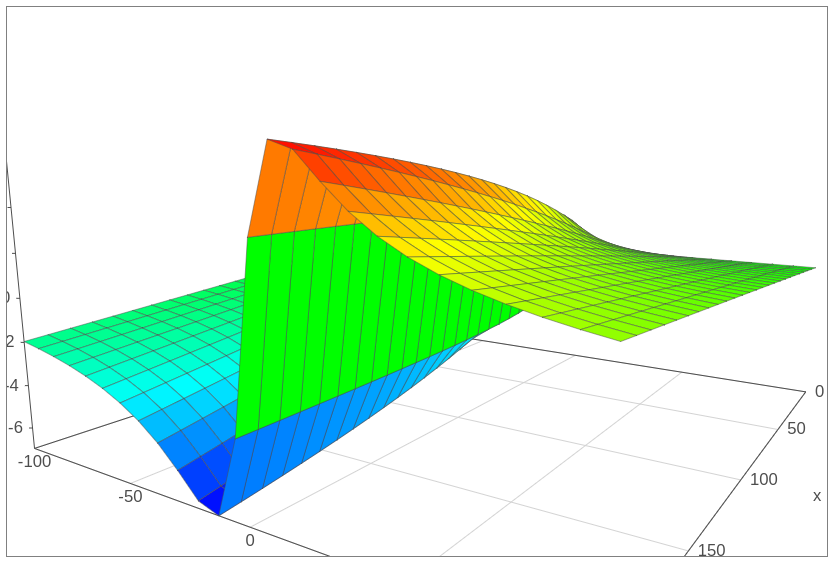
\includegraphics[scale=1]{diagrams/update_term_surface.png}
\end{center}
\caption{The 3D surface illustration of the update function $u(x, y)$ }
\label{fig:figure_1}
\end{figure}


Where, $x$ has the role of the instantaneous cost and $y$ behaves as the gradient. The behaviour of this function can be analysed by considering the 3D surface formed by the function (Figure \ref{fig:figure_1}) \footnote{The figure is generated using the online tool \\ \url{https://academo.org/demos/3d-surface-plotter}}. The figure is a still shot of the surface from an explanatory angle. It is evident that the surface tapers toward the $z = 0$ plane as we go away in either directions in the $y-axis$. This means that the update slows down if the slope becomes too much, i.e. too steep; a behaviour that is desired. Also, the surface cuts the $z = 0$ plane exactly at $y = 0$. This shows that the equation is stable and will converge when the derivative becomes $0$. Finally, the most important feature is that the properties of these taped curves are controlled by the $x$ dimension. As the cost becomes $0$, the $z$ approaches a singularity, i.e. when both $x = 0$ and $y = 0$, the function produces a $\frac{0}{0}$ form. Mathematically,
\begin{center}
		$$\lim_{x \to 0, y \to 0} \left(u(x, y)\right) = \cfrac{xy}{x + y^2} = \phi$$
\end{center}

The point where this singularity occurs, i.e. $(x=0, y=0)$, is the point of global minimum, where the cost is $0$ (a root) and the derivative being $0$ ensures a smooth touch of the cost function to the parameter dimensions' plane. The chances of reaching this point are very less. Through the experimental simulations, it was observed that in the context of computer based numerics, the updated parameters in spite of being ridiculously close, never exactly reach this point due to the round-off effect. The subsequent sub section sheds further light over this phenomenon. Although it is not required, but to ensure numerical safety, a very small value similar to the Adam optimizer can be added to the denominator. This modifies the function as,
\begin{center}
	$z = u(x, y) = \cfrac{xy}{x + y^2 + \epsilon}; \epsilon \leq 10^{-8}$
\end{center}

The addition of the $\epsilon$ gives an oscillating nature to the algorithm. When the algorithm reaches very close to the point of the global minimum (the singularity), the values of the parameters would just oscillate in the $\epsilon$ delta range and would never yeild the $\frac{0}{0}$ value. This is the reason why the $\epsilon$ value has to be very small in order to achieve a good enough approximation.

Another way to visualize the update function $u(x, y)$ is by comparing it with the gradient descent update term. Upon equivalence comparison of the update terms of the two algoriths, it can be deduced that,
\begin{center}
	$\alpha = \cfrac{f(x_t)}{f(x_t) + \left(\cfrac{df(x_t)}{dx}\right)^2}$
\end{center}

This equation yeilds the geometric approximation of the \textit{learning rate} of the gradient descent algorithm. At every iteration $t$ of the proposed algorithm, it emulates the gradient descent behaviour by automatically approximating a value of the step-size (\textit{learning rate}) and uses the sign and magnitude of the instantaneous slope (given by derivative) to make an update.

\subsection{Simulation on single variable synthetic functions}
The proposed algorithm was tested on numerous single variable mathematical functions. This section provides the results obtained on two of those functions. First function is the square function since it is very well behaved, i.e. continuous and differentiable function, corresponding to a preliminary \textit{best-case}. The second function discussed here is the exponential function which represents the most skewed continuous function. It is important to test the algorithm on the $e^x$ function due to its property of being immune to differentiation.

\subsubsection{Square function}
\begin{center}
	Let, $y = f(x) = x^2$ be the objective function
\end{center}

\begin{figure}[h]
\begin{center}
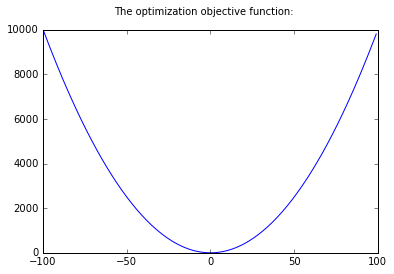
\includegraphics[scale=0.5]{diagrams/square_function.png}
\end{center}
\caption{2D $y$ v/s $x$ plot of the square objective function}
\label{fig:figure_2}
\end{figure}

Upon simulating the proposed algorithm on this function with an initial point $x = 1000$ for just $150$ iterations, the following instantaneous cost plot was obtained (Figure \ref{fig:figure_3}). 

\begin{figure}[h]
\begin{center}
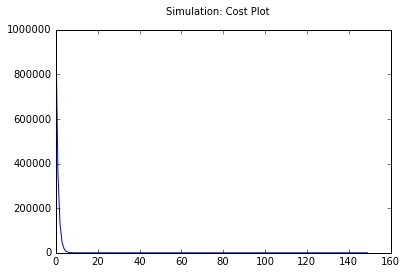
\includegraphics[scale=0.5]{diagrams/ranik_on_square.png}
\end{center}
\caption{2D Cost v/s Iteration plot of the simulation on square function}
\label{fig:figure_3}
\end{figure}

Final optimised position and cost were:\\
$x = 5.493336358815607$ x $10^{-16}$\\
$y = 3.0176743$ x $10^{-31}$\\

for the theoretical (actual) expected values of $x = 0$ and $y = 0$. While, the algorithm reached the $x$ value of the order of $10^{-3}$ in just the initial 30 iterations.

\subsubsection{Exponentiation function}
\begin{center}
	Let, $y = f(x) = e^x$ be the objective function
\end{center}

\begin{figure}[h]
\begin{center}
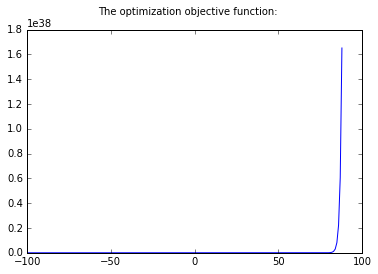
\includegraphics[scale=0.5]{diagrams/exponentiation_function.png}
\end{center}
\caption{2D $y$ v/s $x$ plot of the exponentiation objective function}
\label{fig:figure_4}
\end{figure}

Simulating the same algorithm on the exponentiation function this time, with an initial point $x = 10$ for $100$ iterations, yielded the following instantaneous cost plot (Figure \ref{fig:figure_5}). 

\begin{figure}[h]
\begin{center}
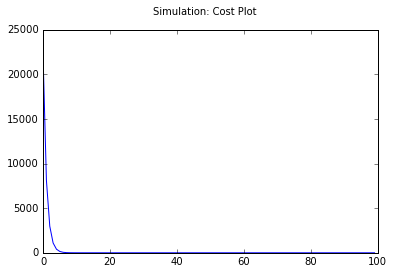
\includegraphics[scale=0.5]{diagrams/ranik_on_exponentiation.png}
\end{center}
\caption{2D Cost v/s Iteration plot of the simulation on exponentiation function}
\label{fig:figure_5}
\end{figure}

with the final optimised position and cost being:\\
$x = -4.47519719694$\\
$y = 0.0115184$\\

for the theoretical (actual) expected values of $x = -\infty$ and $y = 0$.

The function $f(x) = e^x$ has an oblique property of being unchanged by the differentation operator, i.e. 
\begin{center}
	$\cfrac{d(e^x)}{dx} = e^x$
\end{center}
In spite of which, the algorithm proved it's stability during simulation and displayed consistent behaviour in the numerical calculations. Unfortunately the initial position for $x$ could not be set higher, due to the inability of the programming framework to handle values of the order of $e^{20}$.

\section{Experimentation}
In order to test the practical soundness of the proposed algorithm, it was tested on the \textbf{MNIST} \footnote{\url{http://yann.lecun.com/exdb/mnist/}} dataset, which is regarded as the \textit{'Drosophila'} of Machine Learning \cite{goodfellow-et-al:deep-learning}. The classifier that is used is a $3$ layers deep Neural Network having hidden representation size of $512$ dimensions with ReLU activation function \cite{nair:relu}. The use of batch normalization \cite{ioffe:batch-normalization} is avoided since the network is quite shallow and the input data is normalised. The data distribution wouldn’t shift too much in just three layers giving enough scope for ReLU to create non-linear boundaries. No regularization has been employed since the focus is on the optimization part and not the generalisation of the classification. The optimization was performed in the mini-batch gradient descent settings with a batch size of $64$.

The programming implementation of this experiment and the simulations in the previous section are made using the TensorFlow framework \cite{abadi:tensorflow} and have been made open source at the repository [\url{link}] \footnote{For anonymity, the link has been redacted.}. The loss plot shown in (Figure \ref{fig:figure_6}) is obtained after running the algorithm for 12 epochs. The important configuration of the algorithm that needs to be mentioned here is the initialization of the weights. This experiment uses the Xavier initializer \cite{glorot:xavier}.

\begin{figure}[h]
\begin{center}
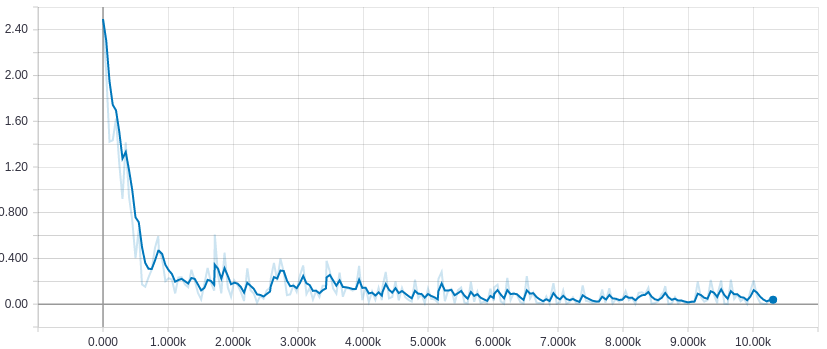
\includegraphics[scale=1.2]{diagrams/ranik_xavier_paper.png}
\end{center}
\caption{2D Cost v/s Iteration plot of the described experiment}
\label{fig:figure_6}
\end{figure}

(Figure \ref{fig:figure_7}) denotes that the performance of the proposed algorithm is comparable to Adam Optimization. This brings to highlight that recently, a number of problems with the Adam optimizer have been highlighted \cite{anonymous:adam-problem}, of which the most prominent being that adam is not guaranteed to converge. Due to which, the analysis of the proposed algorithm becomes more pronounced.

\begin{figure}[h]
\begin{center}
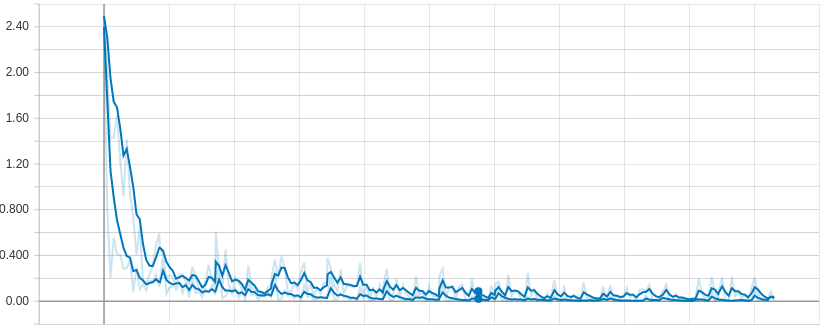
\includegraphics[scale=1.2]{diagrams/ranik_vs_adam_paper.png}
\end{center}
\caption{Comparison of Cost plots of the proposed algorithm and the Adam Optimizer}
\label{fig:figure_7}
\end{figure}

The proposed algorithm was compared alongside a number of other optimizers (more details in [\url{link}]), see (Figure \ref{fig:figure_8}) and it was observed that, majority of the other optimizers without careful tuning of their hyperparameters perfrom a lot worse than the proposed algorithm.

\begin{figure}[h]
\begin{center}
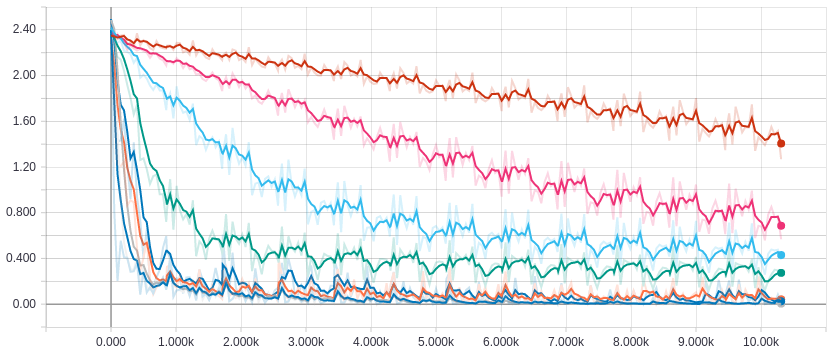
\includegraphics[scale=1.2]{diagrams/ranik_vs_all_paper.png}
\end{center}
\caption{Comparison of Cost plots of the proposed algorithm and other prevailing optimizers}
\label{fig:figure_8}
\end{figure}

\begin{figure}[h]
\begin{center}
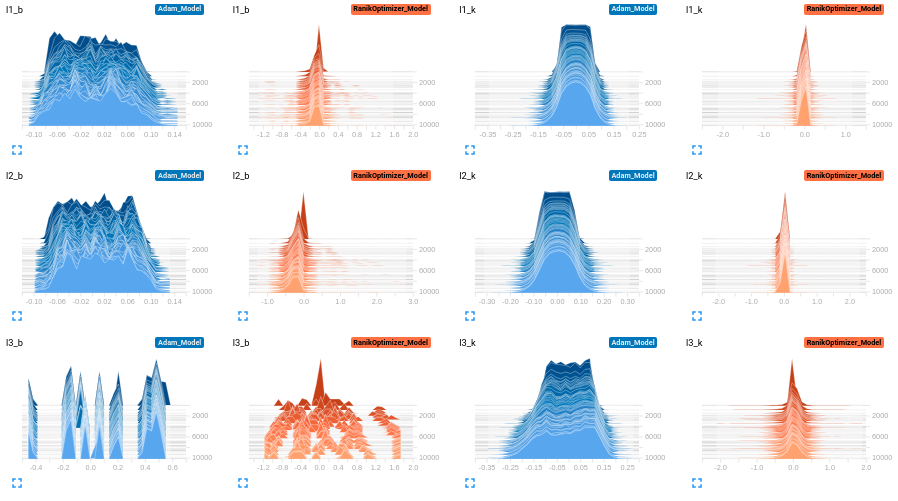
\includegraphics[width=1.0 \linewidth]{diagrams/histograms_ranik_tn_paper.png}
\end{center}
\caption{Histograms of the distributions of the trainable parameters in the Network}
\label{fig:figure_9}
\end{figure}


Another key distinction that is observed as described in (Figure \ref{fig:figure_9}) is that the distribution of the trained parameters for the proposed algorithm resemble the \textbf{\textbf{Laplacian Distribution}} as opposed to the \textbf{\textit{Gaussian Distribution}} trained by the Adam Optimizer.

\section{Conclusions}
The research attempts to establish a hypothesis that the \textit{'dimensions of the objective function and the constituent parameters are relative'}, and paves way for future analysis of this hypothesis. Given the promising results in the described experiments it would be interesting to see haw far can it go for bigger models such as CNN, ResNet, RNN etc. for other more robust Deep Learning datasets. The proposed algorithm without employing any \textit{momentum}, or \textit{RMSprop} mechanisms and utilising simple geometric approximations, achieves performance  comparable to the optimizers that use \textit{momentum }and \textit{RMSprop}. With this, it is urged that the further research in this direction should give more importance to simplicity.

% In the unusual situation where you want a paper to appear in the
% references without citing it in the main text, use \nocite
% \nocite{langley00}

\bibliography{fafomo}
\bibliographystyle{icml2018}

\end{document}


% This document was modified from the file originally made available by
% Pat Langley and Andrea Danyluk for ICML-2K. This version was created
% by Iain Murray in 2018. It was modified from a version from Dan Roy in
% 2017, which was based on a version from Lise Getoor and Tobias
% Scheffer, which was slightly modified from the 2010 version by
% Thorsten Joachims & Johannes Fuernkranz, slightly modified from the
% 2009 version by Kiri Wagstaff and Sam Roweis's 2008 version, which is
% slightly modified from Prasad Tadepalli's 2007 version which is a
% lightly changed version of the previous year's version by Andrew
% Moore, which was in turn edited from those of Kristian Kersting and
% Codrina Lauth. Alex Smola contributed to the algorithmic style files.
